\section{Freifunk V3}

\begin{frame}{}
    \begin{center}
        Freifunk V3
     \end{center}
\end{frame}

\begin{frame}{Warum?}
    \begin{itemize}
        \item \glqq{}Sofa-Knoten\grqq{} verstopfen das Netz, bringen wenig
        \item Wenig Know-How bei Knoten-Aufsteller
        \item Freifunk $\neq$ gratis Hotspot
        \item Mehr Zusammenarbeit
        \begin{itemize}
            \item[$\rightarrow$] Weniger \glqq{}Sofa-Knoten\grqq{}
            \item[$\rightarrow$] Mehr gegenseitige Vernetzung
        \end{itemize}
    \end{itemize}
\end{frame}

\begin{frame}{Die Idee}
    \begin{itemize}
        \item \only<1>{Neuer keyXchange}
            \only<2>{Nein, quatsch! ;)}
            \only<3>{Kein keyXchange mehr}
        \item<3> Es gibt keine spezielle Freifunk Firmware mehr
        \item<3> Kein automatisches Peering mehr
        \item<3> Dezentrale Gateways
        \item<3> \glqq{}Mesh Wolken\grqq{} mit fertigen Komponenten
    \end{itemize}
\end{frame}

\begin{frame}{Wie?}
    \begin{columns}[T]
        \begin{column}{0.46\textwidth}
            \begin{itemize}
                \item Back to the roots
                \item Nur ein Router mit
                \begin{itemize}
                    \item IP Subnetz(en): DHCP, Radvd, etc
                    \item Routing-Protokoll
                    \item VPN Software
                \end{itemize}
                \item Peerings von Hand über
                \begin{itemize}
                    \item Richtfunk
                    \item VPN
                    \item etc
                \end{itemize}
            \end{itemize}
        \end{column}
        \begin{column}{0.46\textwidth}
            \begin{itemize}
                \item Zugänge über
                \begin{itemize}
                    \item Kabel-Netzwerk
                    \item Access-Points
                \end{itemize}
                \item Kein Batman-adv
                \begin{itemize}
                    \item Google Wifi
                    \item AVM Mesh
                    \item TP-Link Deco
                    \item Ubnt UniFi Mesh
                    \item ... \url{http://lmgtfy.com/?q=wlan+mesh+loesungen}
                \end{itemize}
            \end{itemize}
        \end{column}
    \end{columns}
\end{frame}

\begin{frame}{St. Paul}
    \center
    \only<1>{
        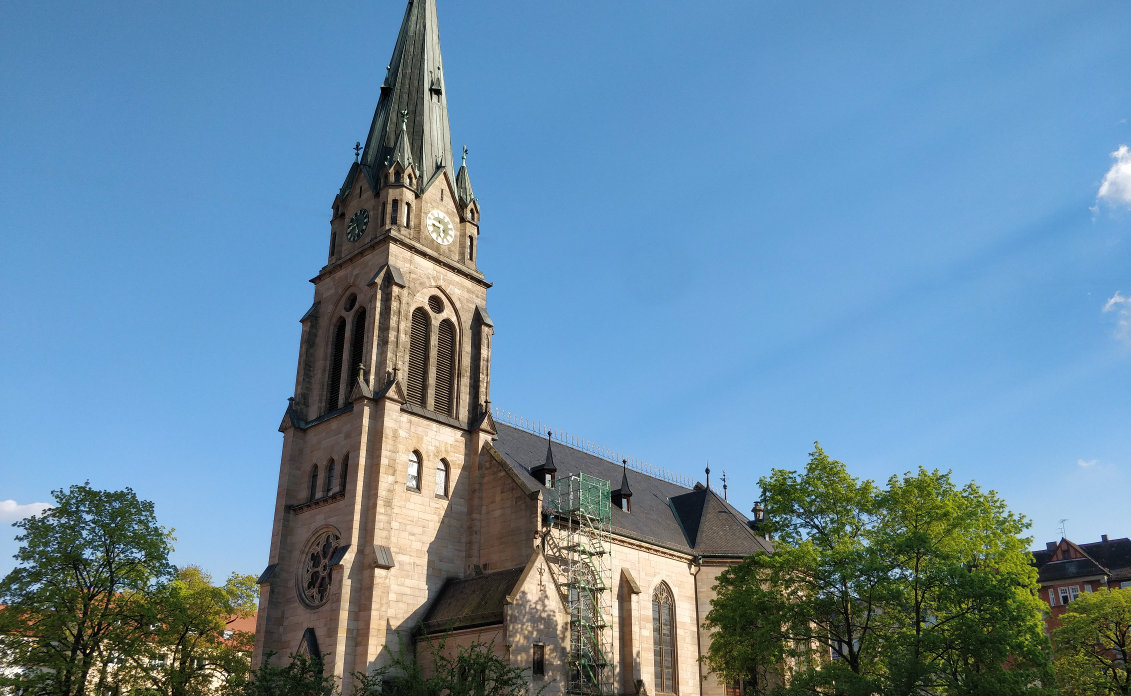
\includegraphics[height=0.86\textheight]{img/stpaul-turm}
    }
    \only<2>{
        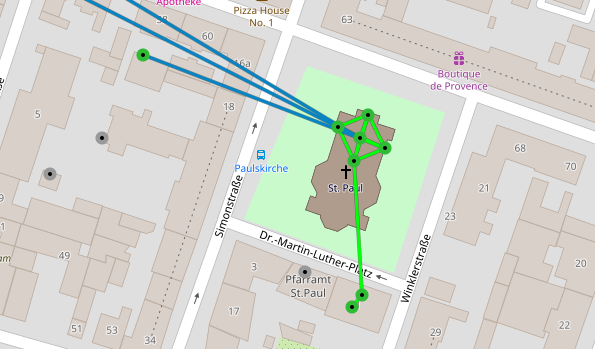
\includegraphics[height=0.86\textheight]{img/stpaul-karte}
    }
    \only<3>{
        \includegraphics[width=0.96\textwidth]{img/dia/stpaul}
    }
    \only<4>{
        ~
        \hfill
        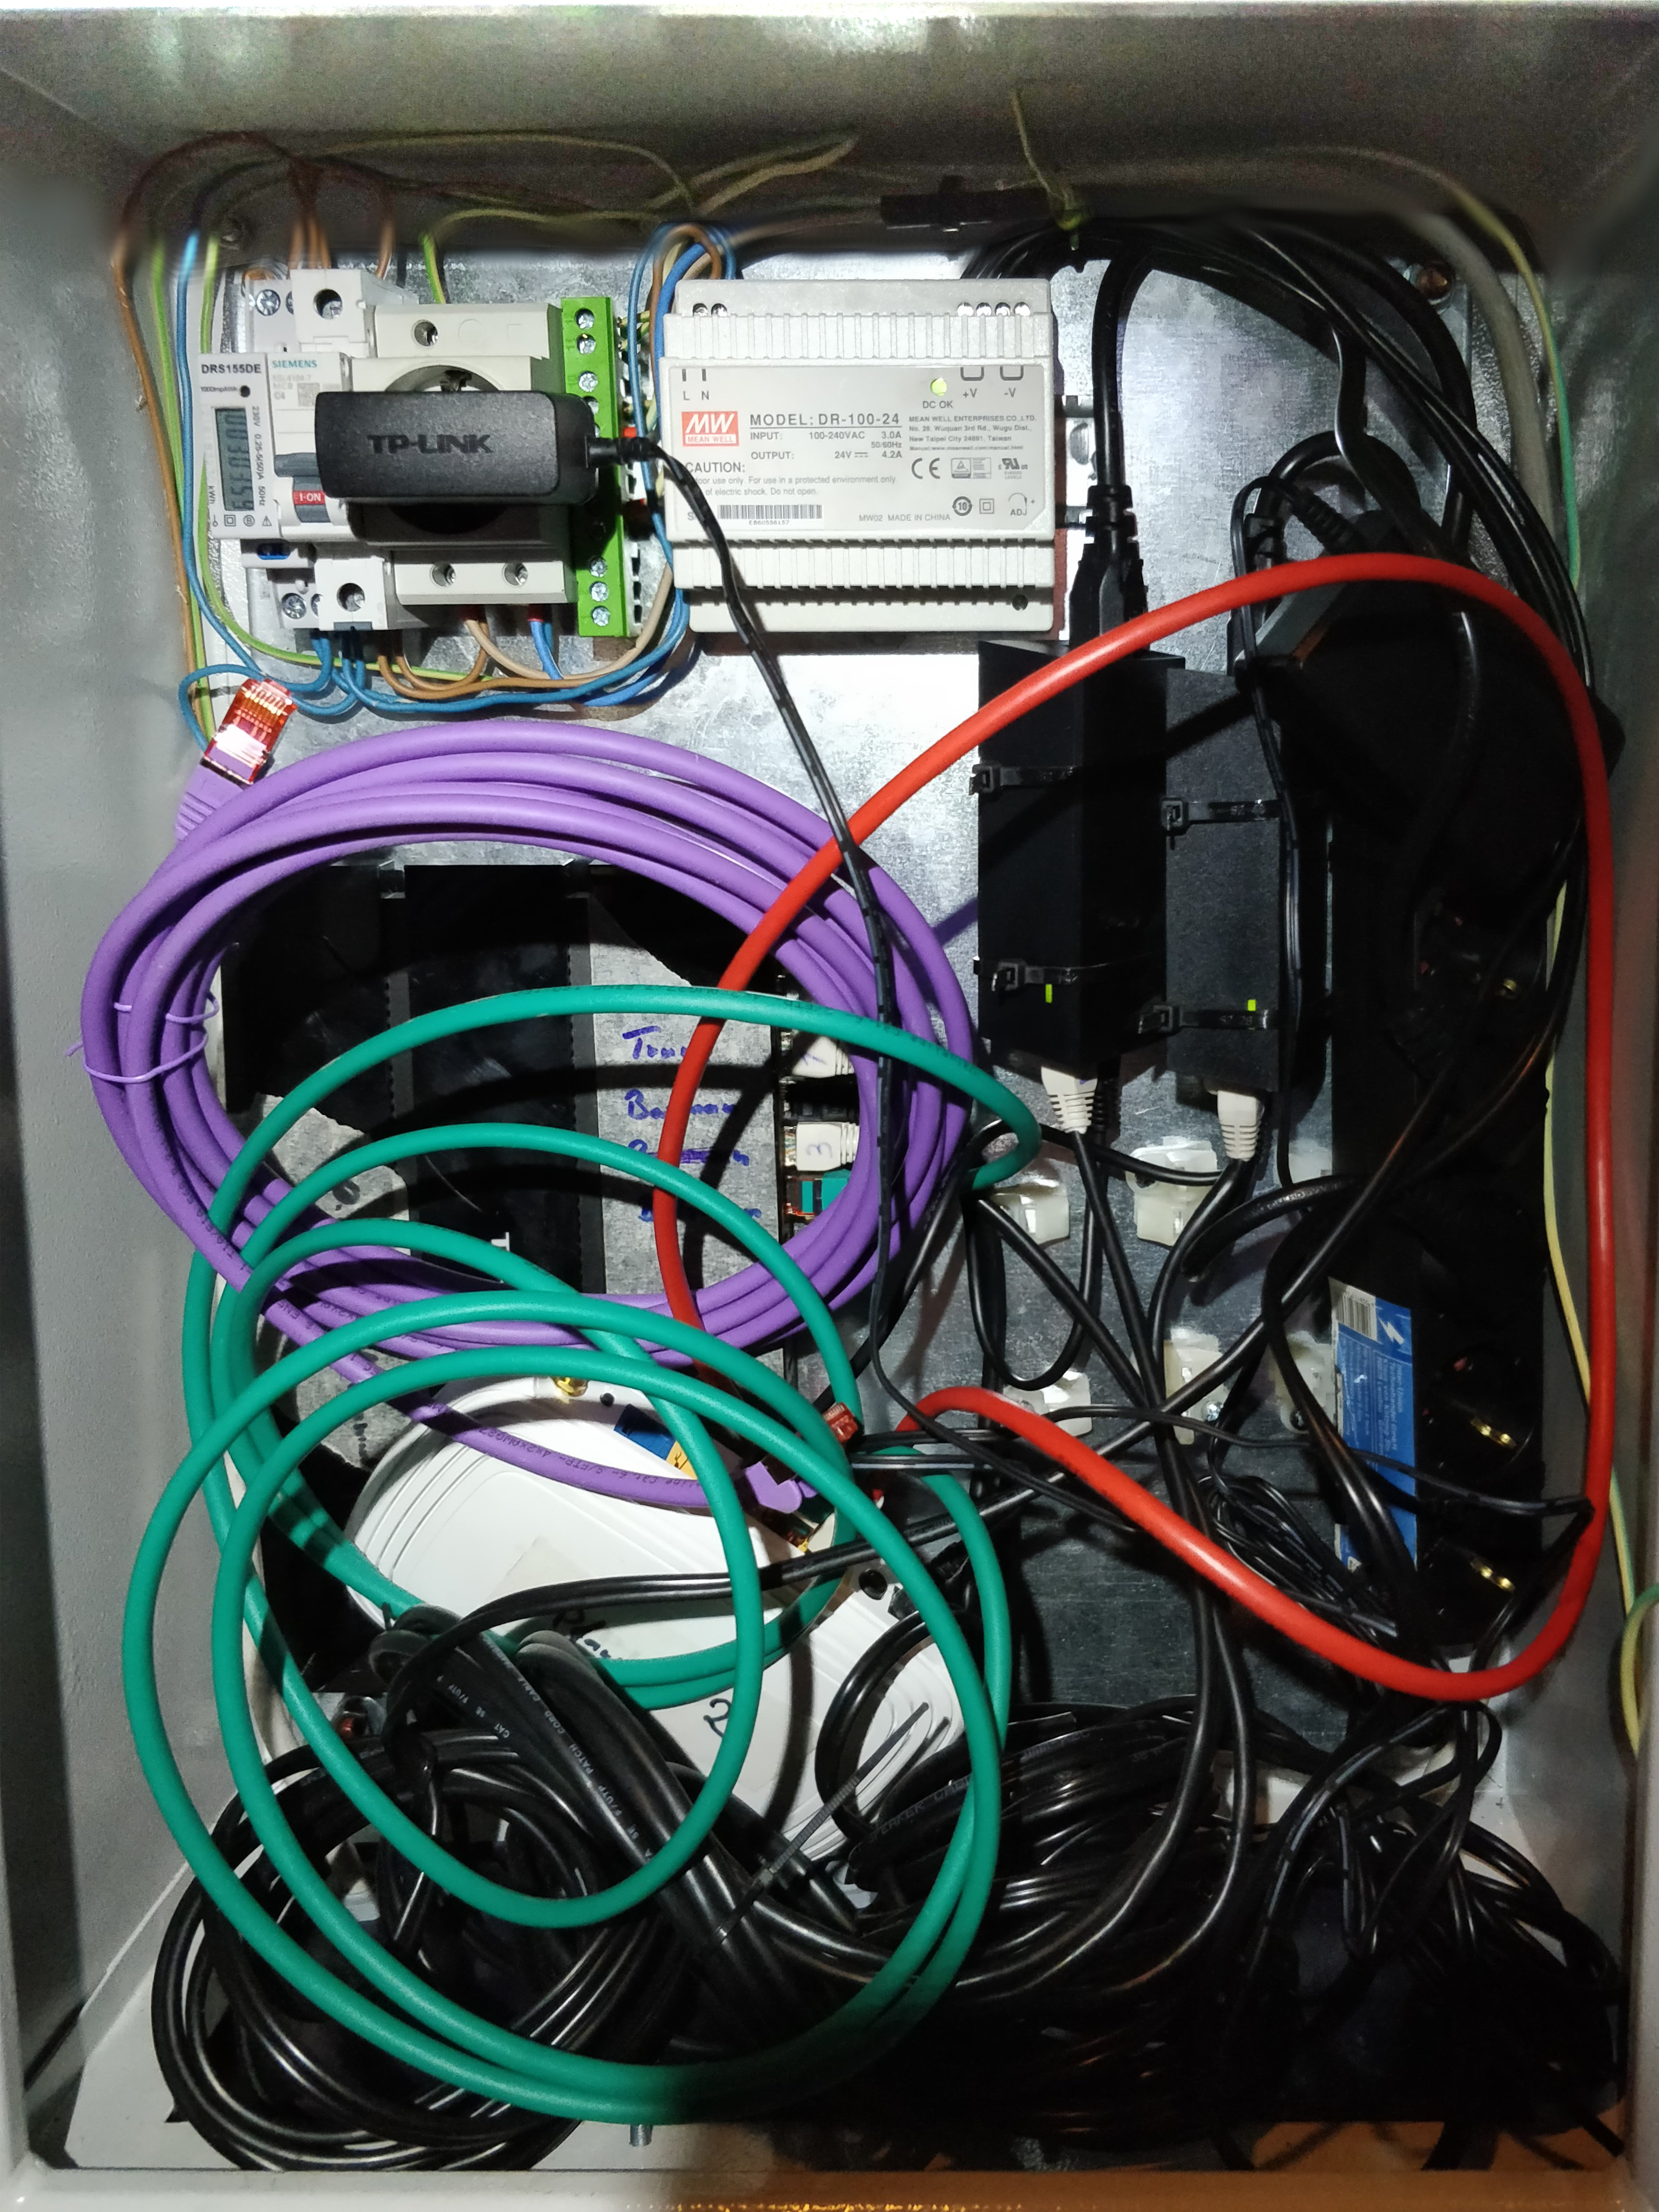
\includegraphics[height=0.86\textheight]{img/stpaul-kasten}
        \hfill
        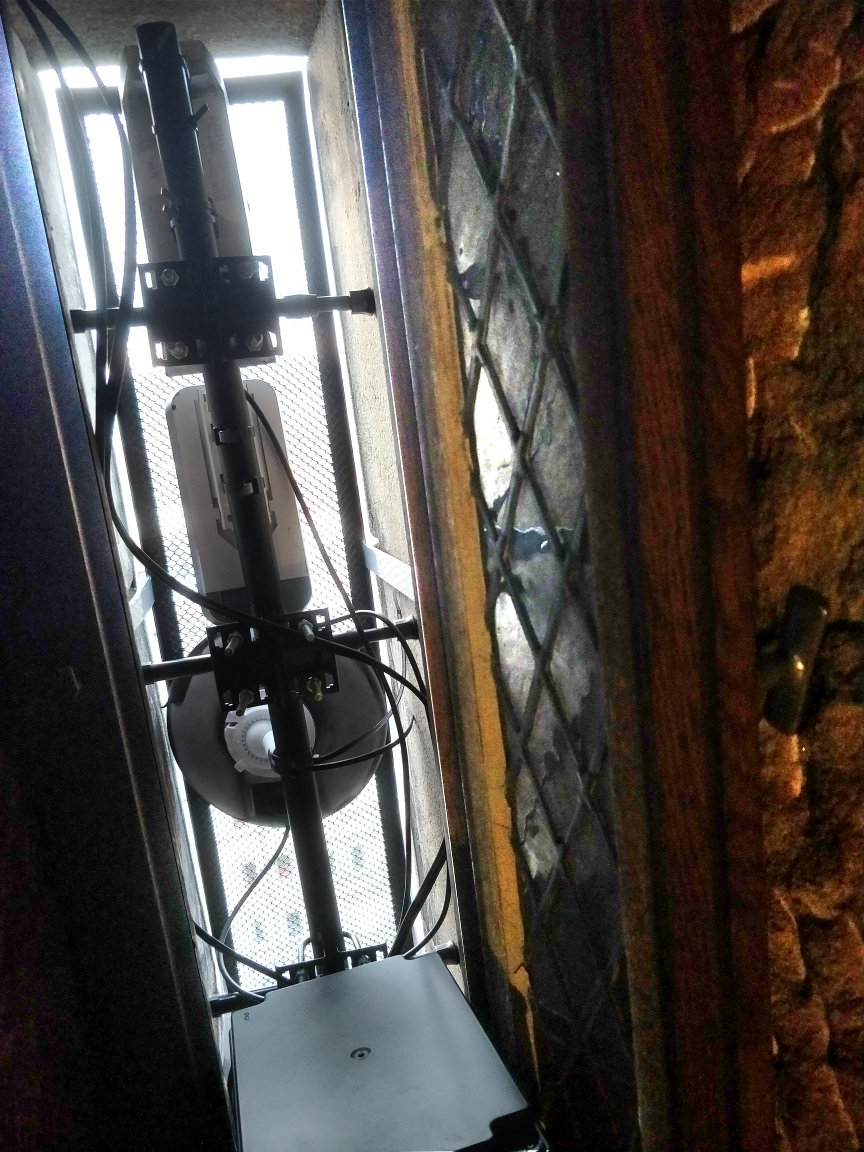
\includegraphics[height=0.86\textheight]{img/stpaul-fenster}
        \hfill
        ~
    }
\end{frame}
